% Options for packages loaded elsewhere
\PassOptionsToPackage{unicode}{hyperref}
\PassOptionsToPackage{hyphens}{url}
\PassOptionsToPackage{dvipsnames,svgnames,x11names}{xcolor}
%
\documentclass[
  authoryear]{elsarticle}

\usepackage{amsmath,amssymb}
\usepackage{iftex}
\ifPDFTeX
  \usepackage[T1]{fontenc}
  \usepackage[utf8]{inputenc}
  \usepackage{textcomp} % provide euro and other symbols
\else % if luatex or xetex
  \usepackage{unicode-math}
  \defaultfontfeatures{Scale=MatchLowercase}
  \defaultfontfeatures[\rmfamily]{Ligatures=TeX,Scale=1}
\fi
\usepackage{lmodern}
\ifPDFTeX\else  
    % xetex/luatex font selection
\fi
% Use upquote if available, for straight quotes in verbatim environments
\IfFileExists{upquote.sty}{\usepackage{upquote}}{}
\IfFileExists{microtype.sty}{% use microtype if available
  \usepackage[]{microtype}
  \UseMicrotypeSet[protrusion]{basicmath} % disable protrusion for tt fonts
}{}
\makeatletter
\@ifundefined{KOMAClassName}{% if non-KOMA class
  \IfFileExists{parskip.sty}{%
    \usepackage{parskip}
  }{% else
    \setlength{\parindent}{0pt}
    \setlength{\parskip}{6pt plus 2pt minus 1pt}}
}{% if KOMA class
  \KOMAoptions{parskip=half}}
\makeatother
\usepackage{xcolor}
\setlength{\emergencystretch}{3em} % prevent overfull lines
\setcounter{secnumdepth}{2}
% Make \paragraph and \subparagraph free-standing
\ifx\paragraph\undefined\else
  \let\oldparagraph\paragraph
  \renewcommand{\paragraph}[1]{\oldparagraph{#1}\mbox{}}
\fi
\ifx\subparagraph\undefined\else
  \let\oldsubparagraph\subparagraph
  \renewcommand{\subparagraph}[1]{\oldsubparagraph{#1}\mbox{}}
\fi


\providecommand{\tightlist}{%
  \setlength{\itemsep}{0pt}\setlength{\parskip}{0pt}}\usepackage{longtable,booktabs,array}
\usepackage{calc} % for calculating minipage widths
% Correct order of tables after \paragraph or \subparagraph
\usepackage{etoolbox}
\makeatletter
\patchcmd\longtable{\par}{\if@noskipsec\mbox{}\fi\par}{}{}
\makeatother
% Allow footnotes in longtable head/foot
\IfFileExists{footnotehyper.sty}{\usepackage{footnotehyper}}{\usepackage{footnote}}
\makesavenoteenv{longtable}
\usepackage{graphicx}
\makeatletter
\def\maxwidth{\ifdim\Gin@nat@width>\linewidth\linewidth\else\Gin@nat@width\fi}
\def\maxheight{\ifdim\Gin@nat@height>\textheight\textheight\else\Gin@nat@height\fi}
\makeatother
% Scale images if necessary, so that they will not overflow the page
% margins by default, and it is still possible to overwrite the defaults
% using explicit options in \includegraphics[width, height, ...]{}
\setkeys{Gin}{width=\maxwidth,height=\maxheight,keepaspectratio}
% Set default figure placement to htbp
\makeatletter
\def\fps@figure{htbp}
\makeatother

\newpageafter{abstract}
\makeatletter
\@ifpackageloaded{tcolorbox}{}{\usepackage[skins,breakable]{tcolorbox}}
\@ifpackageloaded{fontawesome5}{}{\usepackage{fontawesome5}}
\definecolor{quarto-callout-color}{HTML}{909090}
\definecolor{quarto-callout-note-color}{HTML}{0758E5}
\definecolor{quarto-callout-important-color}{HTML}{CC1914}
\definecolor{quarto-callout-warning-color}{HTML}{EB9113}
\definecolor{quarto-callout-tip-color}{HTML}{00A047}
\definecolor{quarto-callout-caution-color}{HTML}{FC5300}
\definecolor{quarto-callout-color-frame}{HTML}{acacac}
\definecolor{quarto-callout-note-color-frame}{HTML}{4582ec}
\definecolor{quarto-callout-important-color-frame}{HTML}{d9534f}
\definecolor{quarto-callout-warning-color-frame}{HTML}{f0ad4e}
\definecolor{quarto-callout-tip-color-frame}{HTML}{02b875}
\definecolor{quarto-callout-caution-color-frame}{HTML}{fd7e14}
\makeatother
\makeatletter
\@ifpackageloaded{caption}{}{\usepackage{caption}}
\AtBeginDocument{%
\ifdefined\contentsname
  \renewcommand*\contentsname{Table of contents}
\else
  \newcommand\contentsname{Table of contents}
\fi
\ifdefined\listfigurename
  \renewcommand*\listfigurename{List of Figures}
\else
  \newcommand\listfigurename{List of Figures}
\fi
\ifdefined\listtablename
  \renewcommand*\listtablename{List of Tables}
\else
  \newcommand\listtablename{List of Tables}
\fi
\ifdefined\figurename
  \renewcommand*\figurename{Figure}
\else
  \newcommand\figurename{Figure}
\fi
\ifdefined\tablename
  \renewcommand*\tablename{Table}
\else
  \newcommand\tablename{Table}
\fi
}
\@ifpackageloaded{float}{}{\usepackage{float}}
\floatstyle{ruled}
\@ifundefined{c@chapter}{\newfloat{codelisting}{h}{lop}}{\newfloat{codelisting}{h}{lop}[chapter]}
\floatname{codelisting}{Listing}
\newcommand*\listoflistings{\listof{codelisting}{List of Listings}}
\makeatother
\makeatletter
\makeatother
\makeatletter
\@ifpackageloaded{caption}{}{\usepackage{caption}}
\@ifpackageloaded{subcaption}{}{\usepackage{subcaption}}
\makeatother
\ifLuaTeX
  \usepackage{selnolig}  % disable illegal ligatures
\fi
\usepackage[]{natbib}
\bibliographystyle{elsarticle-harv}
\usepackage{bookmark}

\IfFileExists{xurl.sty}{\usepackage{xurl}}{} % add URL line breaks if available
\urlstyle{same} % disable monospaced font for URLs
\hypersetup{
  pdftitle={Unravelling mental representations in aphantasia through unsupervised alignment},
  pdfauthor={Maël Delem},
  colorlinks=true,
  linkcolor={blue},
  filecolor={Maroon},
  citecolor={Blue},
  urlcolor={Blue},
  pdfcreator={LaTeX via pandoc}}

\setlength{\parindent}{6pt}
\begin{document}

\begin{frontmatter}
\title{Unravelling mental representations in aphantasia through
unsupervised alignment \\\large{Project design and data analysis
simulation} }
\author[]{Maël Delem%
%
}


        
\begin{abstract}
Research on aphantasia is confronted with a long-standing conundrum of
all research on consciousness and representations, namely the
theoretical inaccessibility of subjective representations. Drawing on
concepts from similarity and representation research, I endorse the view
that the study of an individual's mental representations is made
possible by exploiting second-order isomorphism. The concept of
second-order isomorphism means that correspondence should not be sought
in the first-order relation between (a) an external object and (b) the
corresponding internal representation, but in the second-order relation
between (a) the perceived similarities between various external objects
and (b) the similarities between their corresponding internal
representations. Building on this idea, this study project report is
divided into five parts. \textbf{First}, I outline the central ideas
underlying similarity research and its applicability to aphantasia
research. \textbf{Second}, I present a methodological rationale and
protocol based on inverse multidimensional scaling that can be
implemented online to conduct such large-scale research with high
efficiency. \textbf{Third}, I present a data analysis plan using a
state-of-the-art method for similarity analysis, unsupervised alignment
with Gromov-Wasserstein optimal transport (GWOT). \textbf{Fourth}, I
report a data simulation of a potential outcome of this project and the
successful analysis of this synthetic data using GWOT alignment.
\textbf{Fifth}, I analyse the feasability of such a project given the
material constraints of my thesis. I conclude with the expected utility
and benefits of this project.
\end{abstract}





\end{frontmatter}
    
\renewcommand*\contentsname{Table of contents}
{
\hypersetup{linkcolor=}
\setcounter{tocdepth}{2}
\tableofcontents
}
\begin{tcolorbox}[enhanced jigsaw, bottomrule=.15mm, toptitle=1mm, opacitybacktitle=0.6, left=2mm, rightrule=.15mm, opacityback=0, colbacktitle=quarto-callout-tip-color!10!white, breakable, titlerule=0mm, colback=white, bottomtitle=1mm, coltitle=black, leftrule=.75mm, title=\textcolor{quarto-callout-tip-color}{\faLightbulb}\hspace{0.5em}{Project inception}, arc=.35mm, colframe=quarto-callout-tip-color-frame, toprule=.15mm]

This project stems from several elements:

\begin{enumerate}
\def\labelenumi{\arabic{enumi}.}
\item
  The long standing knowledge of the fact that internal representations
  seem impossible to reach due to their subjective nature.
\item
  The discovery of the article of
  \citet{shepardSecondorderIsomorphismInternal1970} that expose the idea
  of ``second-order isomorphism''.
\item
  The discovery of state-of-the-art and accessible unsupervised analytic
  methods to study this principle in an astonishing way. The last two
  discoveries (and many more) are the fruit of amazing discussions and
  recommendations from Ladislas when he came here. These motivated me to
  try to implement GWOT in R on data that I wanted to create myself to
  emulate a study we could do.
\end{enumerate}

\emph{I promise that I did this mostly on my spare time, we have too
many other things to do elsewhere.}

\end{tcolorbox}

\section{Theoretical context}\label{theoretical-context}

\subsection{Work in progress}\label{work-in-progress}

\subsection{Psychological spaces and
aphantasia}\label{psychological-spaces-and-aphantasia}

While attempting to demonstrate the uselessness of the concept of
similarity as a philosophical and scientific notion\footnote{A claim
  dismissed since then by propositions of robust mathematical models of
  similarity, e.g. \citet{gardenforsConceptualSpacesFramework2004},
  \citet{decockSimilarityGoodman2011}.},
\citet{goodmanSevenStricturesSimilarity1972} has inadvertently expressed
an aspect of similarity judgements of primary importance to us
aphantasia researchers:

\begin{quote}
Comparative judgments of similarity often require not merely selection
of relevant properties but a weighting of their relative importance, and
variation in both relevance and importance can be rapid and enormous.
Consider baggage at an airport checking station. The spectator may
notice shape, size, color, material, and even make of luggage; the pilot
is more concerned with weight, and the passenger with destination and
ownership. Which pieces are more alike than others depends not only upon
what properties they share, but upon who makes the comparison, and when.
. . . Circumstances alter similarities.
\end{quote}

This can be easily reversed as an argument in favor of the
\textbf{potential of similarity analyses to highlight the
inter-individual differences in sensory mental representations}. For
example, should we ask individuals to judge the similarities in shape or
color between various objects, the \emph{differences between the
similarity structures} of individuals will be precisely the most
important phenomenon for us, far less than the constancy between these
structures. If we can account for the context dependence, as we will
propose here with explicit instructions, clever task design, and
hypothesis-neutral analysis, we could overcome the limitations of the
inherently subjective nature of similarity judgements.

This idea of a difference in similarity judgements in aphantasia seems
to transpire in the results of
\citet{bainbridgeQuantifyingAphantasiaDrawing2021} on their drawing
study. They have shown that aphantasics had more schematic
representations during recall, accurate in their spatial positioning,
but with less sensory details. This difference can be seen from two
perspectives: (1) a memory deficit for sensory properties; (2) a
different representational structure of the items in their psychological
spaces. In the latter case, aphantasics would have greater/faster
abstraction of their representation of a perceived scene, reducing the
amount of encoded sensory details unconsciously considered to be
relevant. Both (1) and (2) can theoretically explain the same
behavioural response, i.e.~less sensory elements and correct spatial
recall accuracy in aphantasic drawings, but \textbf{the two have
drastically different consequences on how we define, characterize, and
judge aphantasia.}

The dominant hypothesis seems to be that aphantasics simply have an
episodic or general memory deficit. Conversely, I hypothesize that
aphantasics have different representational structures than phantasics
in certain dimensions of their psychological spaces (notably sensory,
but potentially abstract too). More generally, I hypothesize that the
concept of visual imagery evaluates in reality the continuous spectrum
of representational structures in \emph{sensory} dimensions of
psychological spaces. Mirroring visual imagery, spatial imagery could
also be a rough psychometric evaluation of the continuous spectrum of
structural differences in \emph{conceptual/abstract} dimensions of
psychological spaces. In this view, the psychological space of
aphantasics would constrain internal representations to particularly
abstract forms from a very early stage, thus selectively limiting the
item properties thereafter encoded in long-term memory. In other terms,
\textbf{I hypothesize that aphantasia would not be characterized by an
episodic memory deficit, but by an episodic memory \emph{selectivity}
caused by the specific characteristics of their representational
structures and psychological spaces.} This selectivity would have, as we
already hypothesized several times, benefits and drawbacks.

\citet{gardenforsConceptualSpacesFramework2004} proposed that
differences in psychological (in his terms, conceptual) spaces could
arise from various sources, whether innate, due to learning, or broader
cultural or social differences. All these hypotheses could be coherent
to explain the sources of aphantasia. Nevertheless, the study of these
sources should be the subject of very large-scale or longitudinal
studies, which are out of the scope of this project.

Here, we shall rather attempt to \textbf{develop a method to
characterize the differences in aphantasics' representational structures
and psychological spaces.}

\section{Methodology}\label{methodology}

\citet{roads2024}, in a recent review on the state and perspectives of
similarity research, highlighted two challenges that studies in this
field had to face: (1) The high cost of collecting behavioral data on a
large number of stimuli; (2) The lack of software packages being a high
barrier to entry, making the task of coding models difficult for the
uninitiated.

To solve these problems, we present here two solutions, respectively for
(1) experimental design and (2) data analysis:

\begin{enumerate}
\def\labelenumi{\arabic{enumi}.}
\tightlist
\item
  A recent method to efficiently acquire similarity judgements, the
  ``multiple arrangement of items'' and ``inverse multidimensional
  scaling'' developed by \citet{kriegeskorteInverseMDSInferring2012}.
\item
  An accessible and robust Python toolbox provided by
  \citet{sasakiToolboxGromovWassersteinOptimal2023} to conduct
  unsupervised alignment analysis using Gromov-Wasserstein optimal
  transport.
\end{enumerate}

\subsection{Experimental design}\label{experimental-design}

\subsubsection{Multi-arrangement and inverse multidimensional
scaling}\label{multi-arrangement-and-inverse-multidimensional-scaling}

Assuming a geometric model of representational similarities,
\citet{kriegeskorteInverseMDSInferring2012} developed a
multi-arrangement (MA) method to efficiently acquire (dis)similarity
judgments for large sets of objects. The subject has to perform multiple
arrangements of item subsets adaptively designed for optimal measurement
efficiency and for estimating the representational dissimilarity matrix
(RDM) by combining the evidence from the subset arrangements.

The procedure is illustrated in Figure~\ref{fig-multi-arrangement}.

\begin{figure}

\centering{

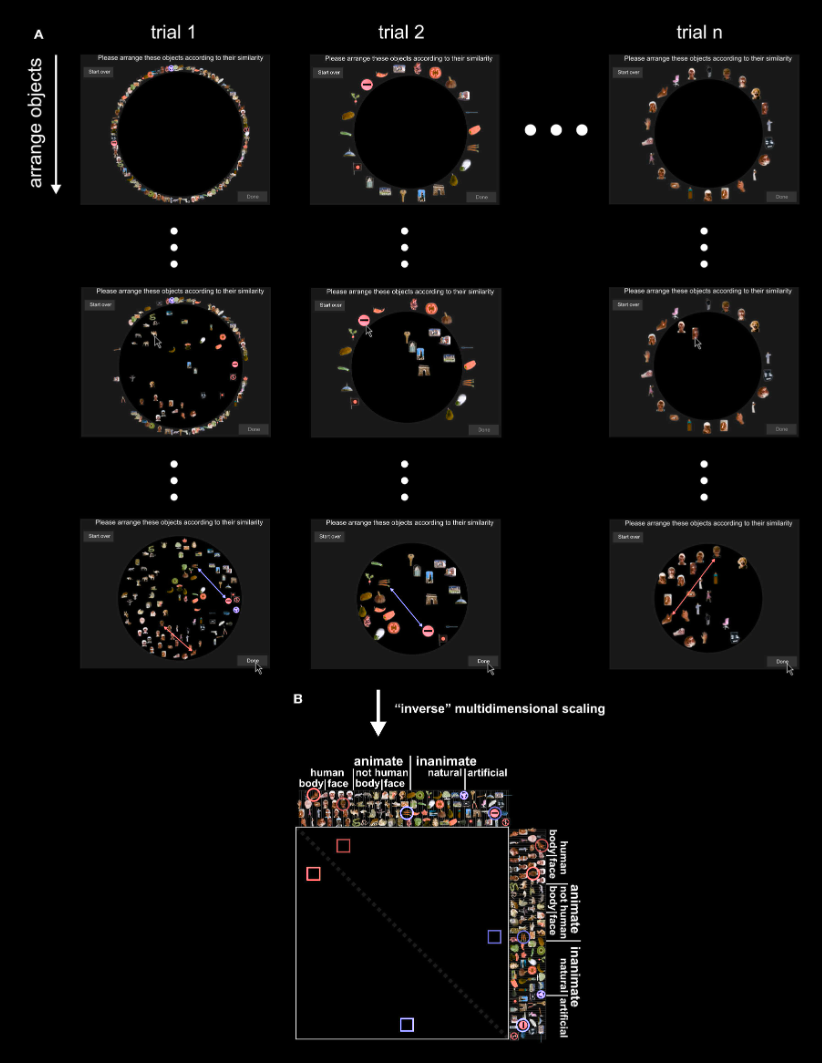
\includegraphics{images/multi-arrangement-method-mur-2013.png}

}

\caption{\label{fig-multi-arrangement}\textbf{Acquiring similarity
judgements with the multi-arrangement method. (A)} Subjects are asked to
arrange items according to their similarity, using mouse drag-and-drop
on a computer. The similarity measure is taken as the distances between
the items: similar items are closer, while dissimilar items are further
apart. The upper part of the figure shows screenshots at different
moments of the acquisition for one subject. Columns are trials and rows
show the object arrangements over time, running from the start (top row)
to the end (last row). The first trial contains all items; subsequent
trials contain subsets of items that are adaptively selected to
optimally estimate judged similarity for each subject. \textbf{(B)} Once
acquisition of the final judgements is completed, inter-item distances
in the final trial arrangements are combined over trials by rescaling
and averaging to yield a single dissimilarity estimate for each object
pair. The process is illustrated in this figure for two example item
pairs: a boy's face and a hand (red), and carrots and a stop sign
(blue). Their single-trial dissimilarity estimates (arrows) are combined
into a single dissimilarity estimate, which is placed at the
corresponding entry of the RDM (lower panel). Mirror-symmetric entries
are indicated by lighter colors \citep[figure
from][]{murHumanObjectSimilarityJudgments2013}.}

\end{figure}%

A key strength of this method that sets it as particularly effective is
the ``adaptive'' part. The goal of the process is to acquire similarity
judgements as precisely as possible while minimizing the total amount of
trials. To do so, starting from the second trial, selected subsets of
the items to be compared are presented to the subject: these items are
the ones that were very close on-screen in previous trials and thus had
their distance evaluated with lower accuracy by the subject. As the
subject has to fill the entire ``arena'' with the items, these
subsequent trials will necessarily increase the level of precision in
the similarity judgement between pairs of items. The second key benefit
of this method is the time and effort gain compared to others. For
example, to compare every pair of items among 64 different items would
require \(\frac{64 \times (64-1)}{2} = 2016\) comparisons (i.e.~trials).
This would be extremely time-consuming, while also losing the
\emph{context-independence} afforded by the MA method due to the
presence of other items around every time the subject mentally performs
a pairwise comparison.

Historically, when referring to the projection of the representations of
stimuli (e.g., coordinates in geometric space) from a high-dimensional
space into a lower-dimensional space, inference algorithms were commonly
called multidimensional scaling \citep{roads2024}. By analogy, the
process of combining several lower-dimensional (2D) similarity
judgements on-screen to form one higher dimensional similarity
representation (in the RDM) can be conceptually seen as ``inverse''
multidimensional scaling, hence the name given to the method by
\citet{kriegeskorteInverseMDSInferring2012}.

\subsubsection{Principle}\label{principle}

The idea is simple: for a given set of items that have distinct and very
pictorial visual properties, we would ask a wide range of aphantasics,
phantasics or hyperphantasics to imagine, mentally compare and make
similarity judgements between the items. To compare these
representations with actual perceptual representations, the subjects
would also perform the same task afterwards, this time with actual
pictures to compare. Subjects would also fill our usual psychometric
imagery questionnaires.

To ``compare imagined items'', we could use a ``word'' version of the MA
paradigm. An example from
\citet{majewskaSpatialMultiarrangementClustering2020} - \emph{who used
the method to build large-scale semantic similarity resources for
Natural Language Processing systems} - is represented in
Figure~\ref{fig-majewska}.

\begin{figure}

\centering{

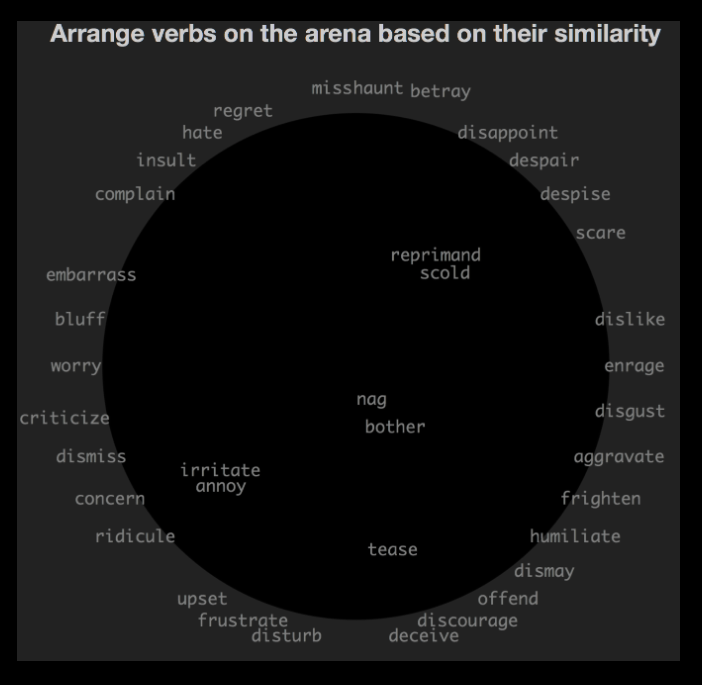
\includegraphics[width=0.5\textwidth,height=\textheight]{images/majewska-spam.png}

}

\caption{\label{fig-majewska}Arena layout of the MA protocol used by to
acquire similarity judgements on word pairs \citep[figure
from][]{majewskaSpatialMultiarrangementClustering2020}.}

\end{figure}%

We could have the stimuli rated by another set of participants on
several features.

\begin{quote}
« \emph{We deliberately did not specify which object properties to focus
on, to avoid biasing participants' spontaneous mental representation of
the similarities between objects. Our aim was to obtain similarity
judgments that reflect the natural representation of objects without
forcing participants to rely on one given dimension. However,
participants were asked after having performed the task, what
dimension(s) they used in judging object similarity.} »
\citep{jozwik2016}
\end{quote}

\begin{quote}
« \textbf{\emph{All but one of the 16 participants reported arranging
the images according to a categorical structure.}} » \citep{jozwik2017}
\end{quote}

This result of \citet{jozwik2017} suggests that we should give an
explicit instruction about the features to focus on, otherwise everyone
might bypass visual features and mental images in favour of concepts and
categories, regardless of their mental imagery profile.

In contrast, if we ask to focus specifically on the visual features,
then ask subjects about the strategy they used to evaluate the
similarities, then on the subjectively felt mental format of these
strategies, we might grasp better insight on the sensory representations
of subjects.

We could even go for several comparisons - even though this would
increase quadratically the number of trials - e.g.~:

\begin{itemize}
\item
  Evaluate to what extent the \textbf{shape} \emph{of these animals are}
  \textbf{\emph{similar}} \textbf{at rest, ignoring size differences.}
\item
  Evaluate to what extent these animals \textbf{sound like each other.}
\item
  Etc.
\end{itemize}

\begin{quote}
\emph{Note to be added: if you do not know the animal, just guess its
placement, as this situation is quite unlikely to happen (animals chosen
are fairly common knowledge).}
\end{quote}

\citet{kawakita2023}: To assess whether the color dissimilarity
structures from different participants can be aligned in an unsupervised
manner, we divided color pair similarity data from a large pool of 426
participants into five participant groups (85 or 86 participants per
group) to obtain five independent and complete sets of pairwise
dissimilarity ratings for 93 color stimuli (Fig. 3a). Each participant
provided a pairwise dissimilarity judgment for a randomly allocated
subset of the 4371 possible color pairs. We computed the mean of all
judgments for each color pair in each group, generating five full
dissimilarity matrices referred to as Group 1 to Group 5.

\subsubsection{Stimuli}\label{stimuli}

We would have a list of animal items, that would have several
characteristics:

\begin{itemize}
\item
  A name
\item
  A category
\item
  A shape
\end{itemize}

We need orthogonal data:

\begin{itemize}
\item
  Each class of animal should include each shape (roughly)
\item
  Each shape should have an animal
\end{itemize}

This would imply that category cannot be derived from shape, and
vice-versa. Thus, a \textbf{sorting by shape would reveal to be innately
visual} (or maybe spatial, if shape concerns this type of imagery), and
a \textbf{sorting by category would reveal an abstraction} from these
shapes. We expect that the two will be mixed to some degree in every
subject, but that low-imagery would rather tend towards category
sorting, while high-imagery would tend towards shape sorting.

Shapes could be very tricky stimuli to discuss. \citet{gardenfors2004}
noted that we only have a very sketchy understanding of how we perceive
and conceptualize things according to their shapes. The works of
\citet{marr1997} highlight this difficulty when analysing the complexity
of the hierarchical judgements of shapes and volumes, as shown in
Figure~\ref{fig-marr}.

\begin{figure}

\centering{

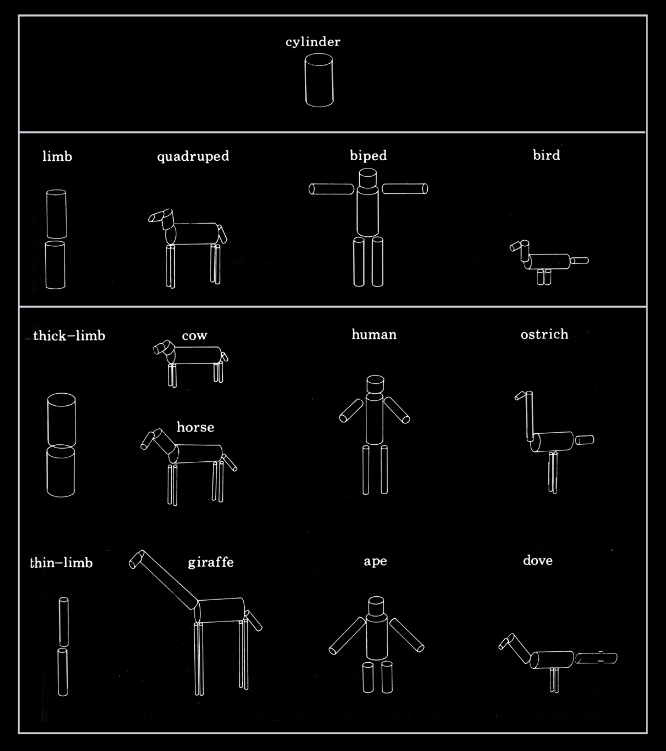
\includegraphics{images/shapes-marr.png}

}

\caption{\label{fig-marr}Representing the characteristics of shapes with
cylinders \citep[figure from][]{marr1997}.}

\end{figure}%

\section{Data analysis plan}\label{data-analysis-plan}

\subsection{Unsupervised alignment
rationale}\label{unsupervised-alignment-rationale}

Visual images can be represented as points in a multidimensional
psychological space. Embedding algorithms can be used to infer latent
representations from human similarity judgments. While there are an
infinite number of potential visual features, an embedding algorithm can
be used to identify the subset of salient features that accurately model
human-perceived similarity. (\emph{From Roads' CV})

Using an optimization algorithm, the free parameters of a psychological
space are found by maximizing goodness of fit (i.e., the loss function)
to the observed data. Historically, when referring specifically to the
free parameters that correspond to the representation of stimuli (e.g.,
coordinates in geometric space), inference algorithms were commonly
called multidimensional scaling (MDS), or simply scaling, algorithms.

In the machine learning literature, analogous inference algorithms are
often called embedding algorithms. The term ``embedding'' denotes a
higher-dimensional representation that is embedded in a
lower-dimensional space. For that reason, the inferred mental
representations of a psychological space could also be called a
psychological embedding.

Numerous techniques exist, and each has limitations. Popular techniques
for comparing representations include RSA \citet{kriegeskorte2008} and
canonical correlation analysis (CCA) (Hotelling 1936). Briefly, RSA is a
method for comparing two representations that assesses the correlation
between the implied pairwise similarity matrices. CCA is a method that
compares two representations by finding a pair of latent variables (one
for each domain) that are maximally correlated.

One might be tempted to compare two dissimilarity matrices assuming
stimulus-level ``external'' correspondence: my ``red'' corresponds to
your ``red''(Fig. 1d). This type of supervised comparison between
dissimilarity matrices, known as Representational Similarity Analysis
(RSA), has been widely used in neuroscience to compare various
similarity matrices obtained from behavioural and neural data. However,
there is no guarantee that the same stimulus will necessarily evoke the
same subjective experience across different participants. Accordingly,
when considering which stimuli evoke which qualia for different
individuals, we need to consider all possibilities of correspondence: my
``red'' might correspond to your ``red'', ``green'', ``purple'', or
might lie somewhere between your ``orange'' and ``pink''(Fig. 1e). Thus,
we compare qualia structures in a purely unsupervised manner, without
assuming any correspondence between individual qualia across
participants.

\subsection{Gromov-Wasserstein optimal
transport}\label{gromov-wasserstein-optimal-transport}

To account for all possible correspondences, we use an unsupervised
alignment method for quantifying the degree of similarity between qualia
structures. As shown in Fig. 2a, in unsupervised alignment, we do not
attach any external (stimuli) labels to the qualia embeddings. Instead,
we try to find the best matching between qualia structures based only on
their internal relationships (see Methods). After finding the optimal
alignment, we can use external labels, such as the identity of a color
stimulus (Fig. 2b), to evaluate how the embeddings of different
individuals relate to each other. This allows us to determine which
color embeddings correspond to the same color embeddings across
individuals or which do not. Checking the assumption that these external
labels are consistent across individuals allows us to assess the
plausibility of determining accurate inter-individual correspondences
between qualia structures of different participants.

To this end, we used the Gromov-Wasserstein optimal transport (GWOT)
method, which has been applied with great success in various fields.
GWOT aims to find the optimal mapping between two point clouds in
different domains based on the distance between points within each
domain. Importantly, the distances (or correspondences) between points
``across'' different domains are not given while those ``within'' the
same domain are given. GWOT aligns the point clouds according to the
principle that a point in one domain should correspond to another point
in the other domain that has a similar relationship to other points. The
principle of the method is illustrated in Figure~\ref{fig-gwot-kawa}

\begin{figure}

\centering{

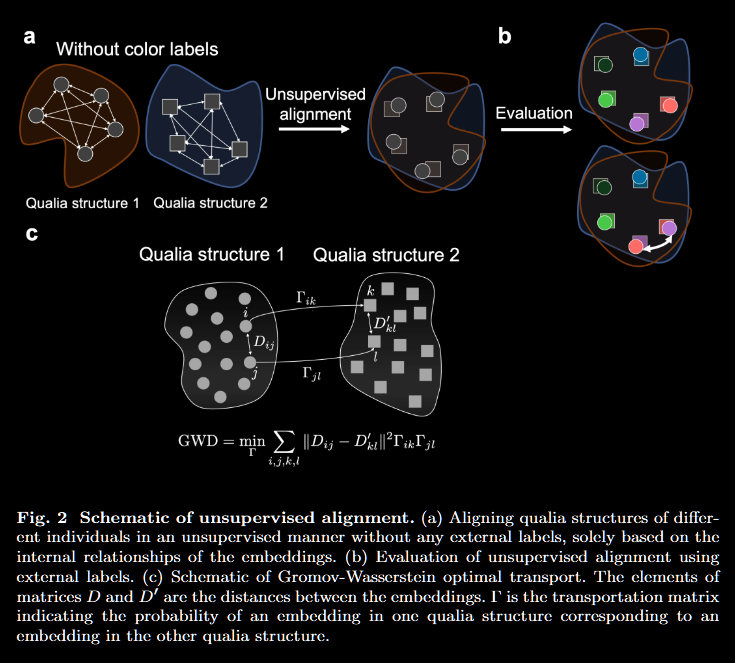
\includegraphics{images/kawa-gwot-2.PNG}

}

\caption{\label{fig-gwot-kawa}Gromov-Wassertein optimal transport
principle \citep[figure from][]{kawakita2023}.}

\end{figure}%

We first computed the GWD for all pairs of the dissimilarity matrices of
the 5 groups (Group 1-5) using the optimized \(\epsilon\). In Fig. 3b,
we show the optimized mapping \(\Gamma*\) between Group 1 and Groups 2-5
(see Supplementary Figure S1 for the other pairs). As shown in Fig. 3b,
most of the diagonal elements in \(\Gamma*\) show high values,
indicating that most colors in one group correspond to the same colors
in the other groups with high probability. We next performed
unsupervised alignment of the vector embeddings of qualia structures.
Although \(\Gamma*\) provides the rough correspondence between the
embeddings of qualia structures, we should find a more precise
mathematical mapping between qualia structures in terms of their vector
embeddings to more accurately assess the similarity between the qualia
structures. Here, we consider aligning the embeddings of all the groups
in a common space.

By applying MDS, we obtained the 3-dimensional embeddings of Group 1 and
Groups 2-5, referred to as X and Yi, where i = 2, \ldots, 5 (Fig. 3c).
We then aligned Yi to X with the orthogonal rotation matrix Qi, which
was obtained by solving a Procrustes-type problem using the optimized
transportation plan \(\Gamma*\) obtained through GWOT (see Methods).
Fig. 3d shows the aligned embed- dings of Group 2-5 (QiYi) and the
embedding of Group 1 (X) plotted in the embedded space of X. Each color
represents the label of a corresponding external color stimulus. Note
that even though the color labels are shown in Fig. 3d, this is only for
the visualization purpose and the whole alignment procedure is performed
in a purely unsupervised manner without relying on the color labels. As
can be seen in Fig. 3d, the embeddings of similar colors from the five
groups are located close to each other, indicating that similar colors
are `correctly' aligned by the unsupervised alignment method.

To evaluate the performance of the unsupervised alignment, we computed
the k-nearest color matching rate in the aligned space. If the same
colors from two groups are within the k-nearest colors in the aligned
space, we consider that the colors are correctly matched. We evaluated
the matching rates between all the pairs of Groups 1-5. The averaged
matching rates are 51\% when k = 1, 83\% when k = 3, and 92\% when k =
5, respectively. This demonstrates the effectiveness of the GW alignment
for correctly aligning the qualia structures of different participants
in an unsupervised manner.

However, as can be seen in Fig. 4b, the optimized mapping \(\Gamma*\) is
not lined up diagonally unlike the optimized map- pings between
color-neurotypical participants groups shown in Fig. 3b (see
Supplementary Figure S1 for the other pairs). Accordingly, top k
matching rate between Group 1-5 and Group 6 is 3.0\% when k = 1 (Fig.
4c), which is only slightly above chance (\(\approx\) 1\%). The matching
rate did not improve even when we relaxed the criterion (6.9\% and 11\%
for k = 3 and k = 5, respectively). Moreover, all of the GWD values
between Group 1-5 and Group 6 are larger than any of the GWD values
between color-neurotypical participant groups (Fig. 4d).

These results indicate that the difference between the qualia structures
of neuro-typical and atypical participants is significantly larger than
the difference between the qualia structures of neuro-typical
participants.

\begin{figure}[H]

{\centering 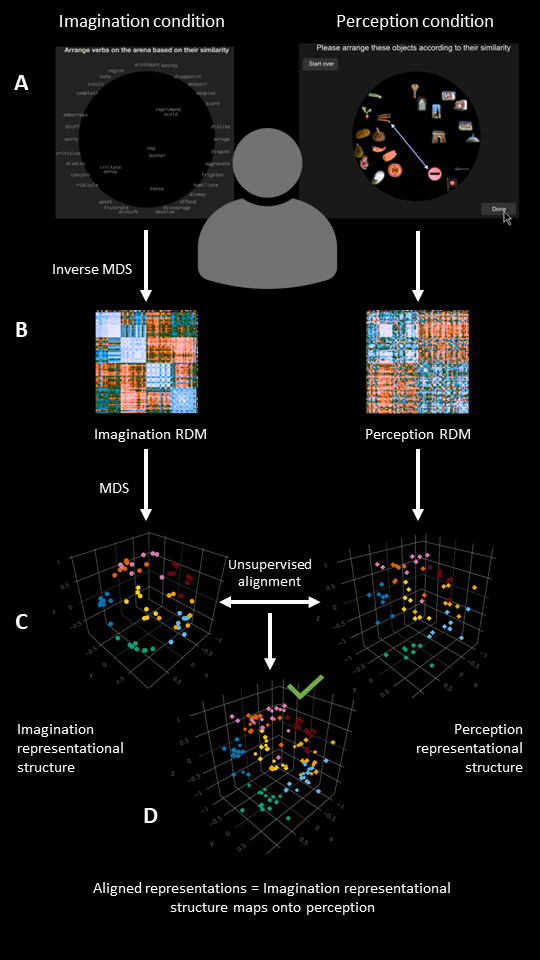
\includegraphics{images/my-protocol-1.png}

}

\caption{The two conditions for one subject.}

\end{figure}%%
\begin{figure}[H]

{\centering 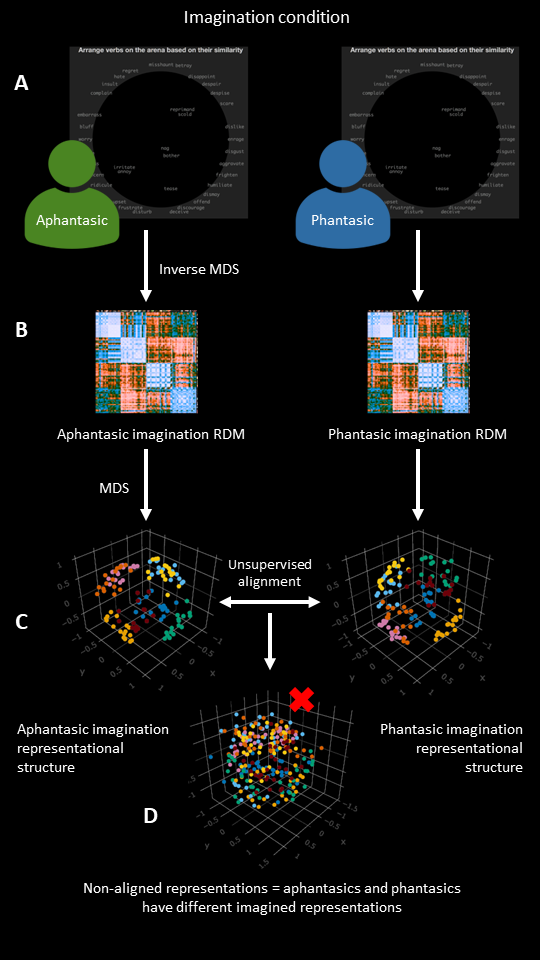
\includegraphics{images/my-protocol-2.png}

}

\caption{The comparison between the representational structure of
aphantasics and phantasics. This figure illustrates the principle, but
in reality all pairs of subjects will be compared to assess their
representational structure alignment. This is computationnally heavy,
but analytically very powerful.}

\end{figure}%

\subsection{Hypotheses}\label{hypotheses}

\subsubsection{Aphantasic and phantasic psychological
spaces}\label{aphantasic-and-phantasic-psychological-spaces}

The most representative members of a category are called prototypical
members.

Prototype theory builds on the observation that among the instances of a
property, some are more representative than others. The most
representative one is the prototype of the property.

Thus, following the concepts illustrated by \citet{gardenfors2004}, we
would expect that aphantasics, when doing shape similarity judgements,
would be more inclined to group items close to the prototypical items
due to a lower definition of the mental image. In comparison, phantasics
would have a much more distributed conceptual space of item shapes due
to their higher-resolution mental images of said items.

\subsubsection{Subjective imagery and psychological
spaces}\label{subjective-imagery-and-psychological-spaces}

In the proposed view of visual imagery as the subjective expression of a
given type of psychological space, we mentioned earlier that
\emph{spatial} imagery could also constitute a subjective expression of
other dimensions of psychological spaces. Hence, the \emph{verbal}
dimension of the simplified model of imagery we outlined in my thesis
project could also represent different dimensions.

This conception leads to the following theoretical hypothesis: provided
that our visual-spatial-verbal model correctly fits subjective imagery,
the imagery profile of individuals should map on their psychological
spaces.

Operationally, this would be evaluated by the fact that
\textbf{individuals with similar imagery profiles} (visual, spatial,
verbal, or any combination of the three) \textbf{should have similar
representations} in their given psychological space,
\textbf{quantifiable by the degree of alignment between their similarity
structures.}

\section{Study simulation and
analysis}\label{study-simulation-and-analysis}

\textsubscript{Source:
\href{https://m-delem.github.io/2499-similarity-manuscript/index.qmd.html}{Article
Notebook}}

\subsection{Visual-spatial-verbal model of cognitive
profiles}\label{visual-spatial-verbal-model-of-cognitive-profiles}

One of the objectives of the study would be to link the subjective
cognitive profiles of individuals with their representational
structures. To evaluate these profiles, we are going to use psychometric
questionnaires evaluating the visual-object, spatial, and verbal
dimensions of imagery which will yield three scores, one for each
dimension.

We are going to simulate 30 participants presenting four different
cognitive profiles, that I defined as, respectively, \emph{verbal}
aphantasics, \emph{spatial} aphantasics, \emph{spatial} phantasics, and
\emph{visual} phantasics. Their imagery abilities are summarised in
Table~\ref{tbl-imageries}.

To simulate these four sub-groups, we use the \texttt{holodeck} R
package to generate multivariate normal distributions of scores on these
three dimensions for each sub-group. For instance, verbal aphantasics
have normally distributed visual imagery scores centered around a mean
of 0 (normalized, so negative scores are possible), 0.4 for spatial
imagery, and 0.7 for verbal style; Spatial aphantasics have means of 0
for visual, 0.75 spatial, and 0.3 for verbal; etc. The numbers are
arbitrary, but have been chosen by trial-and-error to obtain a model
that is both well-defined and not exaggerated. The 30 subjects' imagery
profiles are represented in the three dimensional space of the
visual-spatial-verbal dimensions in Figure~\ref{fig-plot-osv-model}.

\begin{longtable}[]{@{}lccc@{}}
\caption{Imagery abilities of the four hypothesized cognitive
profiles.}\label{tbl-imageries}\tabularnewline
\toprule\noalign{}
Cognitive profile & Visual imagery & Spatial imagery & Verbal style \\
\midrule\noalign{}
\endfirsthead
\toprule\noalign{}
Cognitive profile & Visual imagery & Spatial imagery & Verbal style \\
\midrule\noalign{}
\endhead
\bottomrule\noalign{}
\endlastfoot
Verbal aphantasic & -- & - & ++ \\
Spatial aphantasic & -- & ++ & - \\
Spatial phantasic & + & ++ & - \\
Visual phantasic & ++ & - & + \\
\end{longtable}

\phantomsection\label{cell-fig-plot-osv-model}
\begin{figure}[H]

\centering{

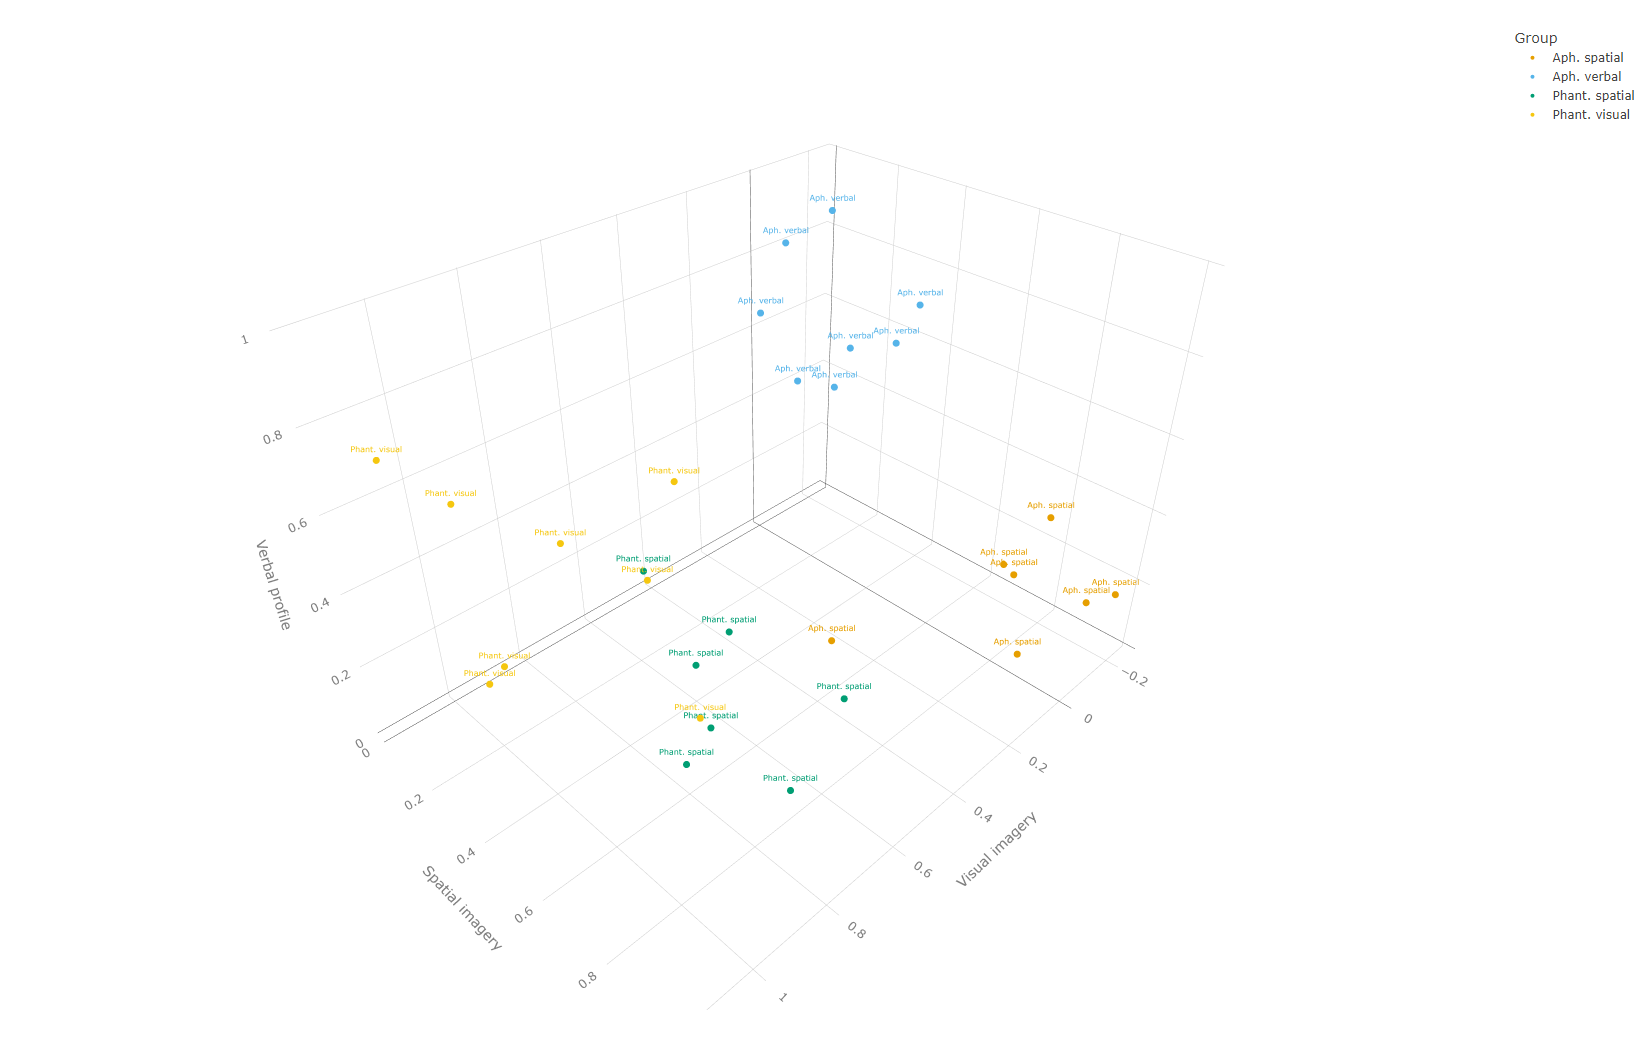
\includegraphics{index_files/figure-pdf/fig-plot-osv-model-1.png}

}

\caption{\label{fig-plot-osv-model}Imagery profiles generated for 30
subjects on the three object, spatial, and verbal dimensions.}

\end{figure}%

\textsubscript{Source:
\href{https://m-delem.github.io/2499-similarity-manuscript/index.qmd.html}{Article
Notebook}}

\subsection{Data simulation: Creating representational
structures}\label{data-simulation-creating-representational-structures}

\citet{gardenfors2004} invokes two scientific concepts, to wit,
prototypes and Voronoi tessellations. Prototype theory builds on the
observation that among the instances of a property, some are more
representative than others. The most representative one is the prototype
of the property. \emph{We hypothesize that aphantasics will be more
inclined to categorize items according to prototypes than phantasics.}

A Voronoi tesselation of a given space divides that space into a number
of cells such that each cell has a center and consists of all and only
those points that lie no closer to the center of any other cell than to
its own center; the centers of the various cells are called the
generator points of the tesselation. This principle will underlie our
data simulation, as we will build representations in a 3D space based on
distances to ``centroids'', namely, prototypes. These representations
will thus be located inside of the tessellations around these
prototypes, more or less close to the centroid depending on the
subject's representational structures.

\subsubsection{Generating ``prototype'' embeddings from a
sphere}\label{generating-prototype-embeddings-from-a-sphere}

\textsubscript{Source:
\href{https://m-delem.github.io/2499-similarity-manuscript/index.qmd.html}{Article
Notebook}}

A function will be used to generate embeddings. These spherical
embeddings are displayed in Figure~\ref{fig-perfect-embeddings} We get 8
nicely distributed clusters. We'll retrieve the centroids of each
cluster, which would be the ``perfect'' categories of each species group
(say, generated by a computational model on categorical criteria).

\phantomsection\label{cell-fig-perfect-embeddings}
\begin{figure}[H]

\centering{

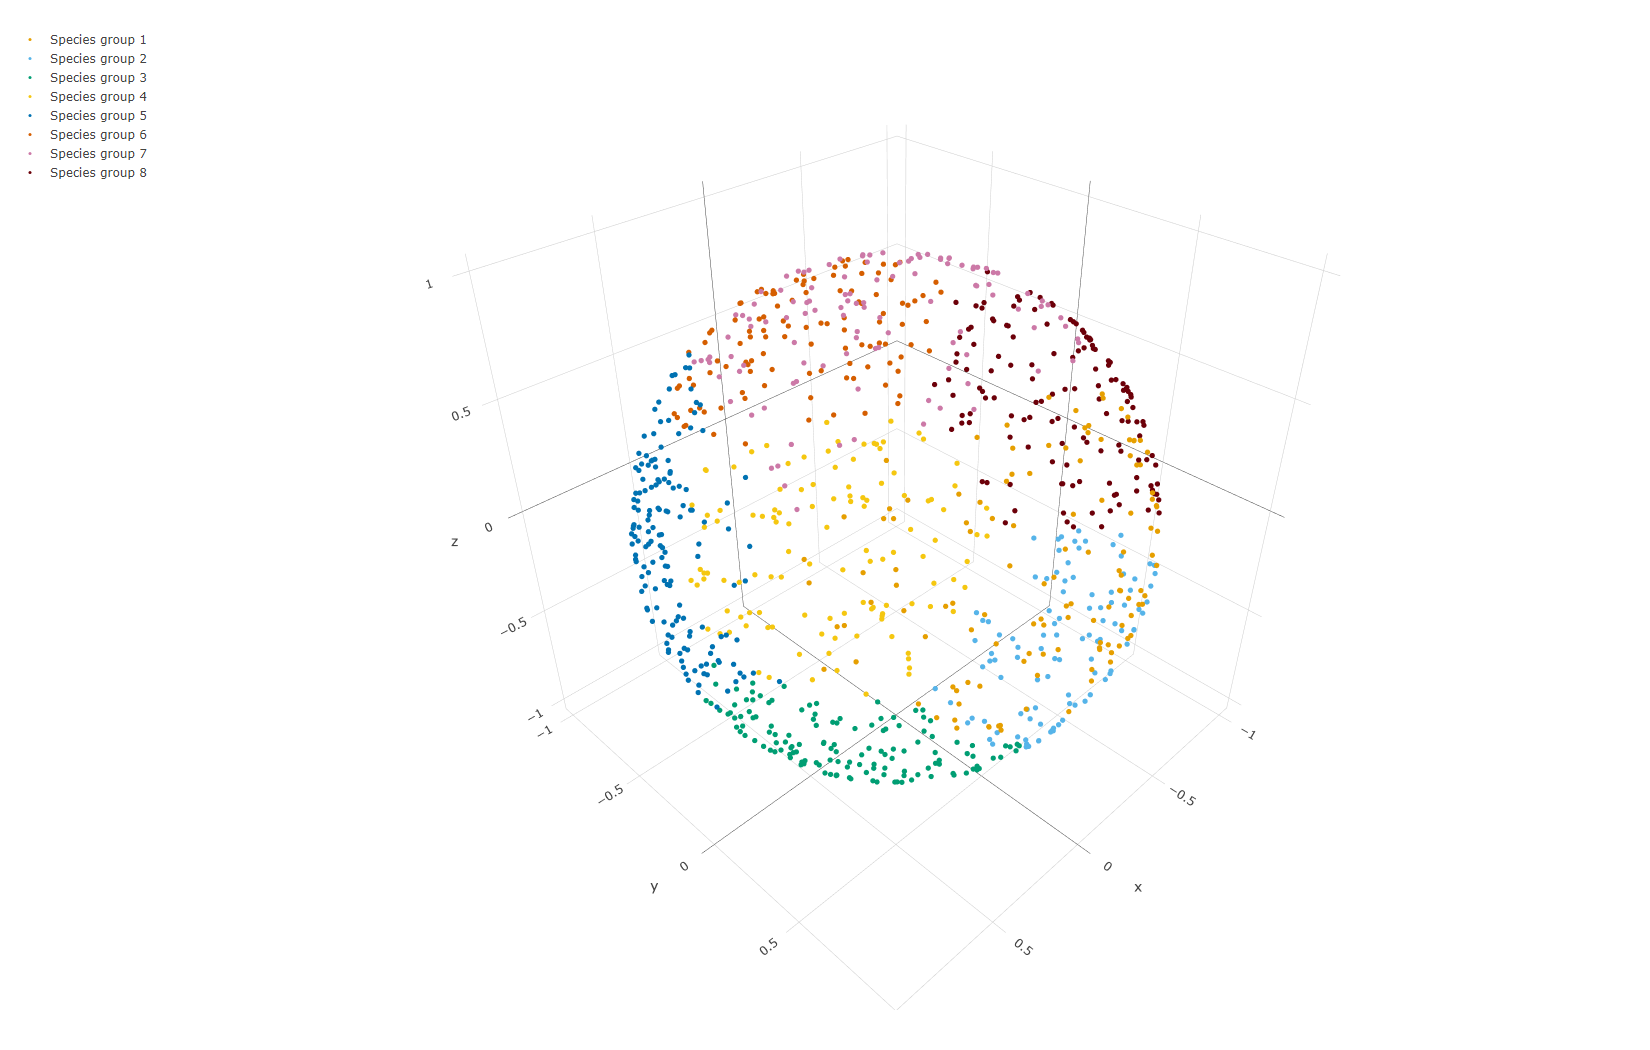
\includegraphics{index_files/figure-pdf/fig-perfect-embeddings-1.png}

}

\caption{\label{fig-perfect-embeddings}Generated spherical distribution
of 1000 observations grouped in 8 equal clusers with Gaussian Mixture
Clustering to represent the theoretical embeddings of 8 groups
(i.e.~groups of species here). \textbf{\emph{Interact with the figures
to see the details.}}}

\end{figure}%

\textsubscript{Source:
\href{https://m-delem.github.io/2499-similarity-manuscript/index.qmd.html}{Article
Notebook}}

\phantomsection\label{cell-fig-centroids}
\begin{figure}[H]

\centering{

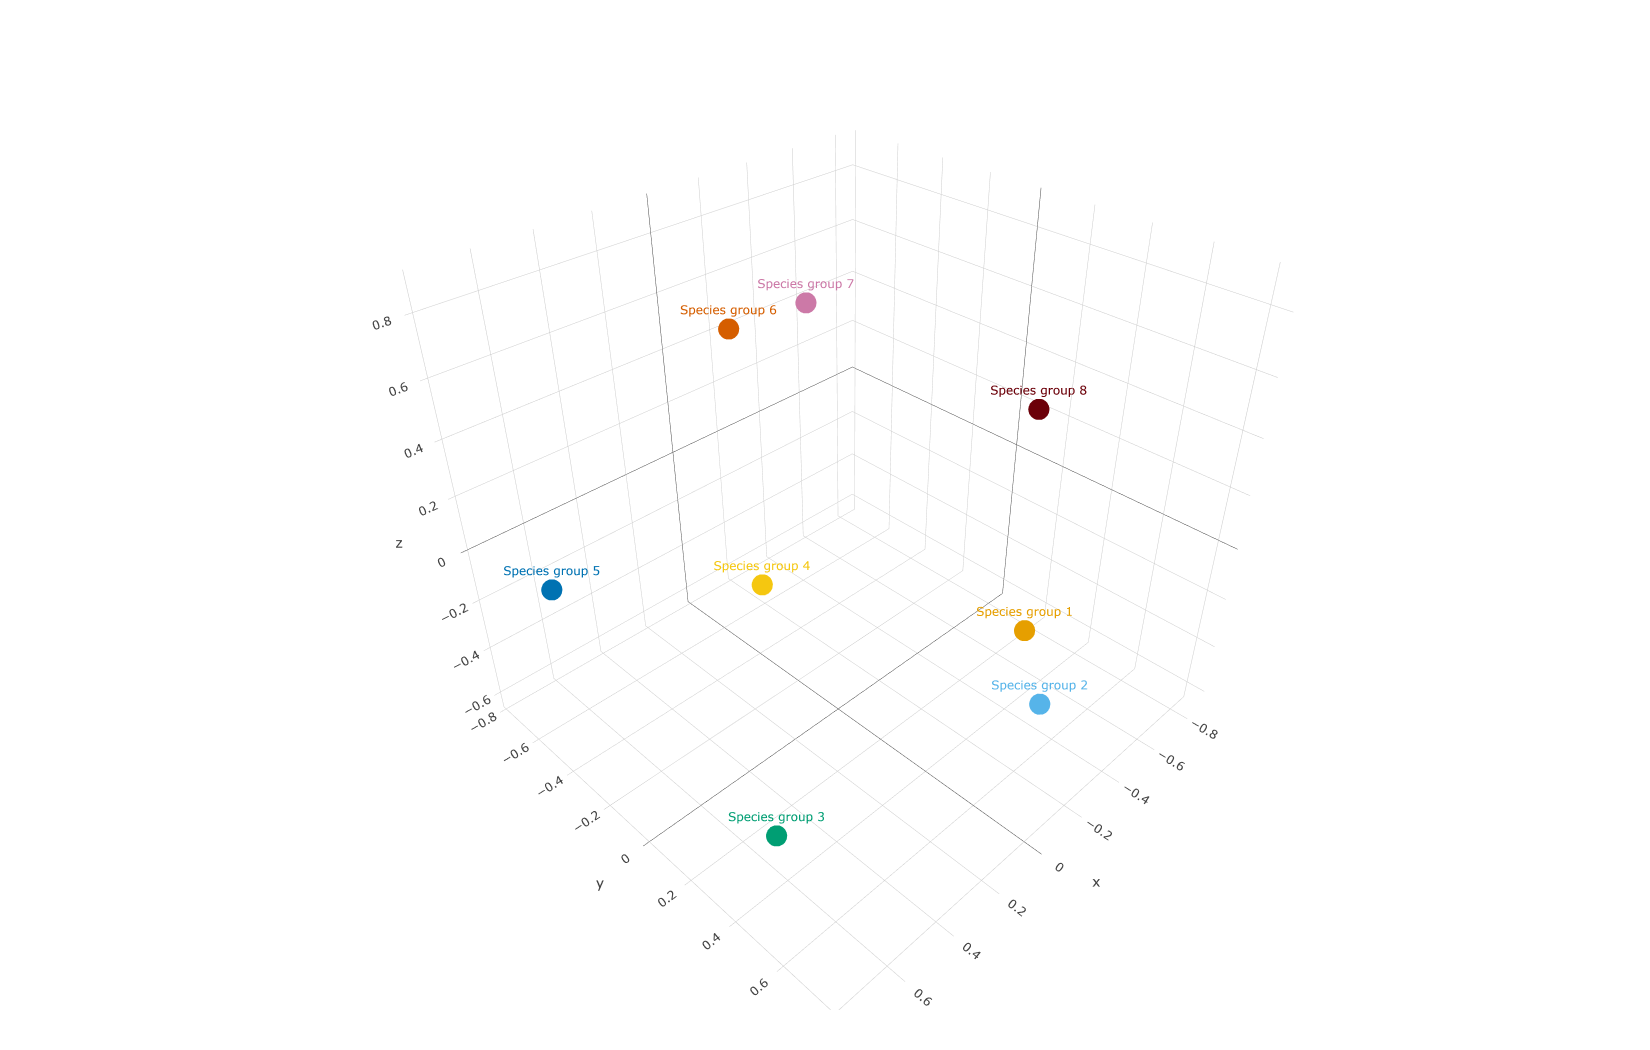
\includegraphics{index_files/figure-pdf/fig-centroids-1.png}

}

\caption{\label{fig-centroids}Centroids of the 8 clusters created on the
sphere, thus representing the prototypical embeddings of 8 groups
(i.e.~groups of species here). \textbf{\emph{Interact with the figures
to see the details.}}}

\end{figure}%

\textsubscript{Source:
\href{https://m-delem.github.io/2499-similarity-manuscript/index.qmd.html}{Article
Notebook}}

Now we want two sets of embeddings: one where the observations are very
concentrated around the centroids, which would be the
\textbf{categorical model}, and one where the observations are more
spread out, which would be the \textbf{visual model}.

We need to select 8 observations per cluster, which would be our animals
per group. These observations will be subsets of the 1000 observations
we generated.

\subsubsection{Categorical model
embeddings}\label{categorical-model-embeddings}

The selection procedure for the \textbf{categorical model} will consist
of selecting points that are rather \emph{close to the centroids}. Thus,
we will filter the observations of the large sets to keep only points
for which the distance to the centroid is inferior to a given value.
That is, points for which the Euclidean norm of the vector from the
observation to the centroid:

\[d(centroid, observation) = \sqrt{(x_{c} - x_{o})^{2} + (y_{c} - y_{o})^{2} + (z_{c} - z_{o})^{2}}\]

This can be done using the function
\texttt{norm(coordinates,\ type\ =\ "2")} in R.

\phantomsection\label{cell-fig-categorical-embeddings}
\begin{figure}[H]

\centering{

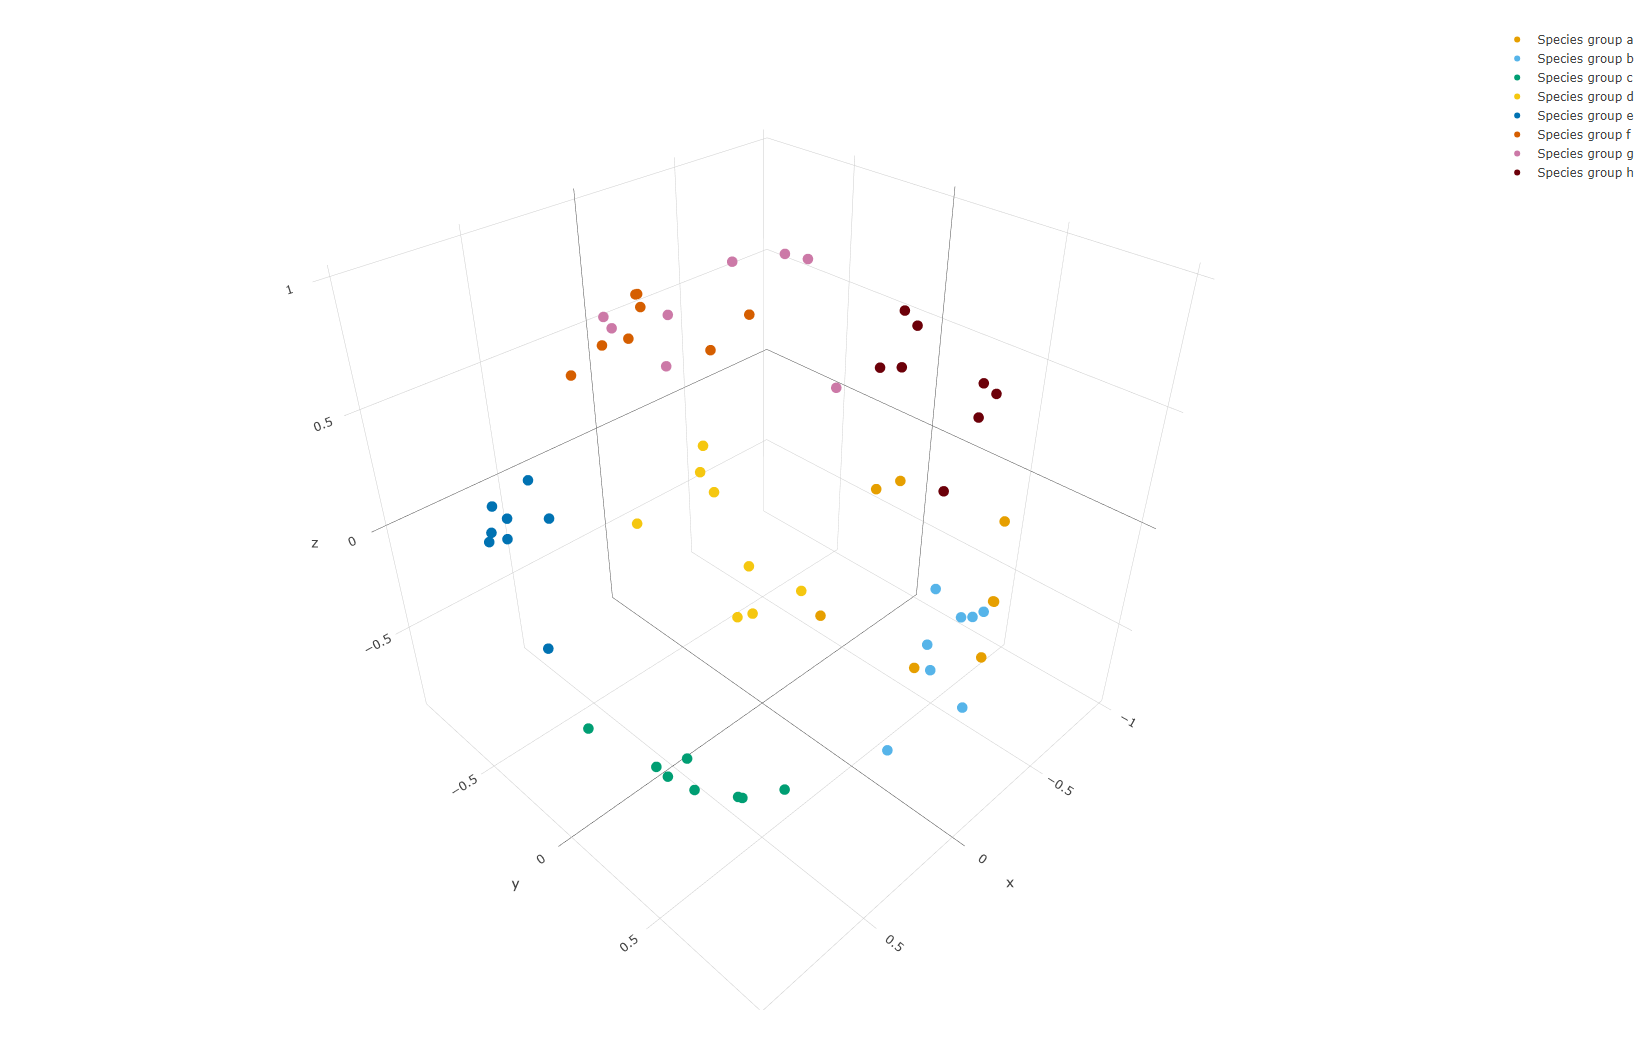
\includegraphics{index_files/figure-pdf/fig-categorical-embeddings-1.png}

}

\caption{\label{fig-categorical-embeddings}Selection of 64 points to
represent prototypical categorical embeddings, based on the distances to
each groups' centroid. These will be the bases of the verbal
aphantasics' embeddings. \textbf{\emph{Interact with the figure to see
the details.}}}

\end{figure}%

\textsubscript{Source:
\href{https://m-delem.github.io/2499-similarity-manuscript/index.qmd.html}{Article
Notebook}}

\subsubsection{Visual model embeddings}\label{visual-model-embeddings}

In the case of the \textbf{visual model}, we would like approximately
evenly distributed embeddings, that could also dive \emph{inside} the
sphere, i.e.~representing species that are visually close although
diametrically opposed when it comes to taxonomy. To do this we could try
to simulate multivariate normal distributions around the
centroids\footnote{A simpler alternative would be generating the visual
  embeddings with the same code as the categorical ones, selecting 8
  points per cluster but much more spread out (e.g.~selecting 8 among
  the 90\% closest to the centroids, which would create more variability
  than the categorical one set to 60\%). I chose otherwise because this
  wouldn't have had points reaching \emph{inside} the sphere.}. This can
be done with the \texttt{holodeck} package.

\phantomsection\label{cell-fig-visual-embeddings}
\begin{figure}[H]

\centering{

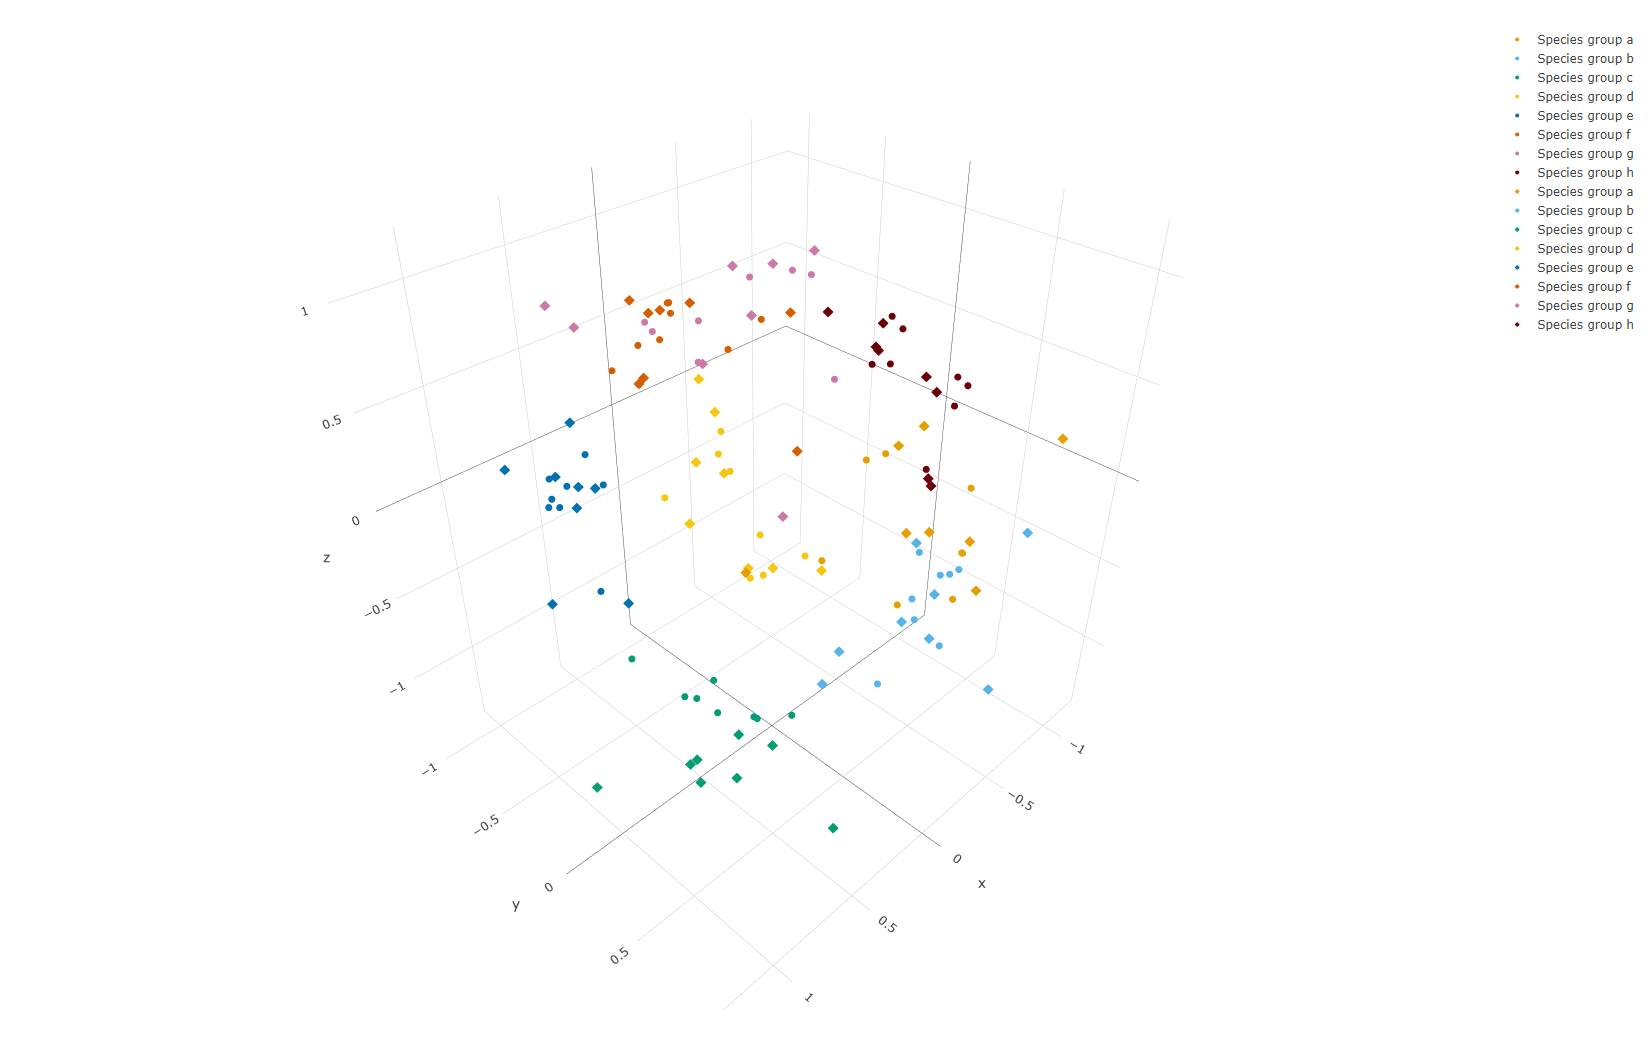
\includegraphics{index_files/figure-pdf/fig-visual-embeddings-1.png}

}

\caption{\label{fig-visual-embeddings}Selection of 64 points to
represent prototypical visual embeddings, chosen randomly in
multivariate distributions centered around each categorical embedding.
The visual embeddings are overlaid as diamonds along with categorical
ones as dots. The two distributions keep the group structure, but are
pretty far apart at times. \textbf{\emph{Interact with the figure to see
the details.}}}

\end{figure}%

\textsubscript{Source:
\href{https://m-delem.github.io/2499-similarity-manuscript/index.qmd.html}{Article
Notebook}}

\subsubsection{Intermediate embeddings}\label{intermediate-embeddings}

\begin{figure}

\centering{

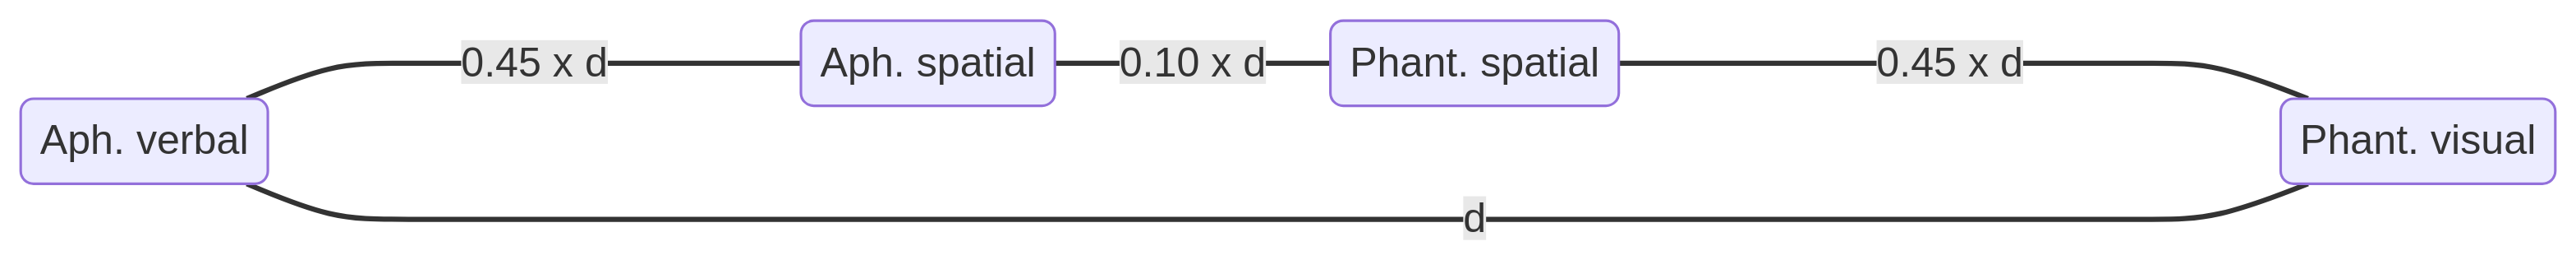
\includegraphics[width=7in,height=0.71in]{index_files/figure-latex/mermaid-figure-3.png}

}

\caption{\label{fig-distances-graph}Model of the distances between
participants' representations. Note that here d is a one-dimensional
distance between the representations, but it will be computed as a
three-dimensional distance in our toy-model. The verbal aphantasic
profile is hypothesized to be very categorical, thus diametrically
opposed to the visual phantasic profile, by a given distance d.~Spatial
profiles are in-between: they are close to each other (10\% x d), but
the spatial aphantasic profile is a bit closer to the verbal aphantasic
one (45\% x d), and the spatial phantasic is a bit closer to the visual
phantasic one (45\% x d).}

\end{figure}%

\textsubscript{Source:
\href{https://m-delem.github.io/2499-similarity-manuscript/index.qmd.html}{Article
Notebook}}

\textsubscript{Source:
\href{https://m-delem.github.io/2499-similarity-manuscript/index.qmd.html}{Article
Notebook}}

\phantomsection\label{cell-fig-intermediate-embeddings}
\begin{figure}[H]

\centering{

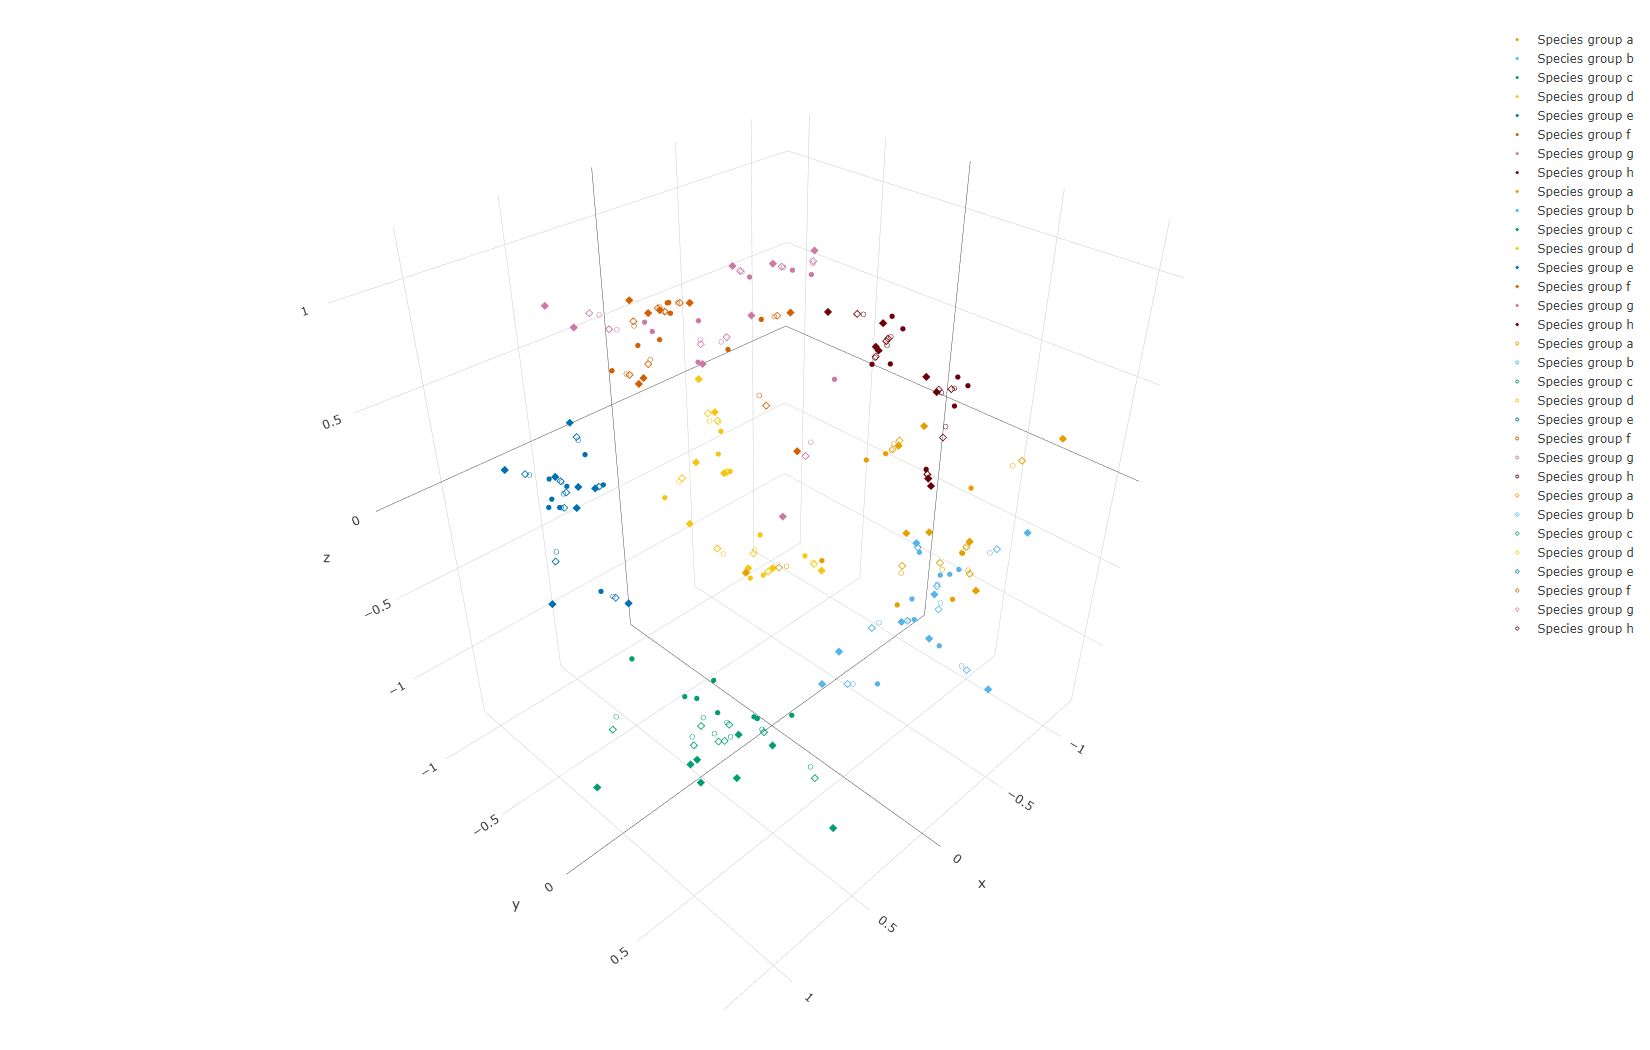
\includegraphics{index_files/figure-pdf/fig-intermediate-embeddings-1.png}

}

\caption{\label{fig-intermediate-embeddings}Space of embeddings with 128
additional points based on the euclidean distances between the visual
and categorical embeddings. The empty dots are the
\emph{aphantasics-spatial} ones, and the empty diamonds are the
\emph{phantasic-spatial} ones. Some can be very close together, and
sometimes further apart due to the various pairs of visual and
categorical points used to create them. A network-like structure seems
to appear, with empty points seemingly `connecting' the dots and
diamonds. \textbf{\emph{Interact with the figure to see the details.}}}

\end{figure}%

\textsubscript{Source:
\href{https://m-delem.github.io/2499-similarity-manuscript/index.qmd.html}{Article
Notebook}}

\subsubsection{Labelling the species}\label{labelling-the-species}

The distributions created are still gathered around the centroids of
each group, but are much more widespread, each group getting close to
each other and even reaching inside the sphere.

Perfect! Now we have two 3D embeddings per animal, in a categorical or a
visual description of their features. Let's add labels for each species
in a group:

\textsubscript{Source:
\href{https://m-delem.github.io/2499-similarity-manuscript/index.qmd.html}{Article
Notebook}}

Now we have four sets of coherent coordinates, that we need to assign to
the 30 participants: i.e.~generating 8 points for C (aph\_spa\_low), 7
points for CS (aph\_spa\_high), 7 points for VS (phant\_spa\_high), and
8 points for V (phant\_spa\_low).

\subsubsection{Generating the subject
embeddings}\label{generating-the-subject-embeddings}

We have four ``reference'' sets of embeddings which represent animals
either judged according to their similarity in categorical terms
(namely, species), or in visual terms (namely shape or color
similarities, assuming that these similarities are more evenly
distributed, e.g.~the crab looks like a spider, but is also pretty close
to a scorpion, etc.).

To generate the embeddings of each subject in each condition, we will
start from these reference embeddings and generate random noise around
\emph{each item}, i.e.~for all 64 animals. For 100 subjects, we would
thus generate 100 noisy points around each animal, each point
corresponding to a given subject.

The visual and verbal groups will be generated with slightly more
intra-group variance, so as to try to make the spatial groups as
coherent as possible (and avoid blurring everything and making the
groups disappear in noise).

Although the groupings in this distribution sound simple when we color
it using the knowledge about how we built it, the algorithm will only be
fed with the data for each subject, without any labeling or additional
information. Thus, Figure~\ref{fig-subject-embeddings-b} here is what
the algorithm will ``see'' (and what it will try to decrypt).
Admittedly, that looks a lot more complicated.

\phantomsection\label{cell-fig-subject-embeddings-a}
\begin{figure}[H]

\centering{

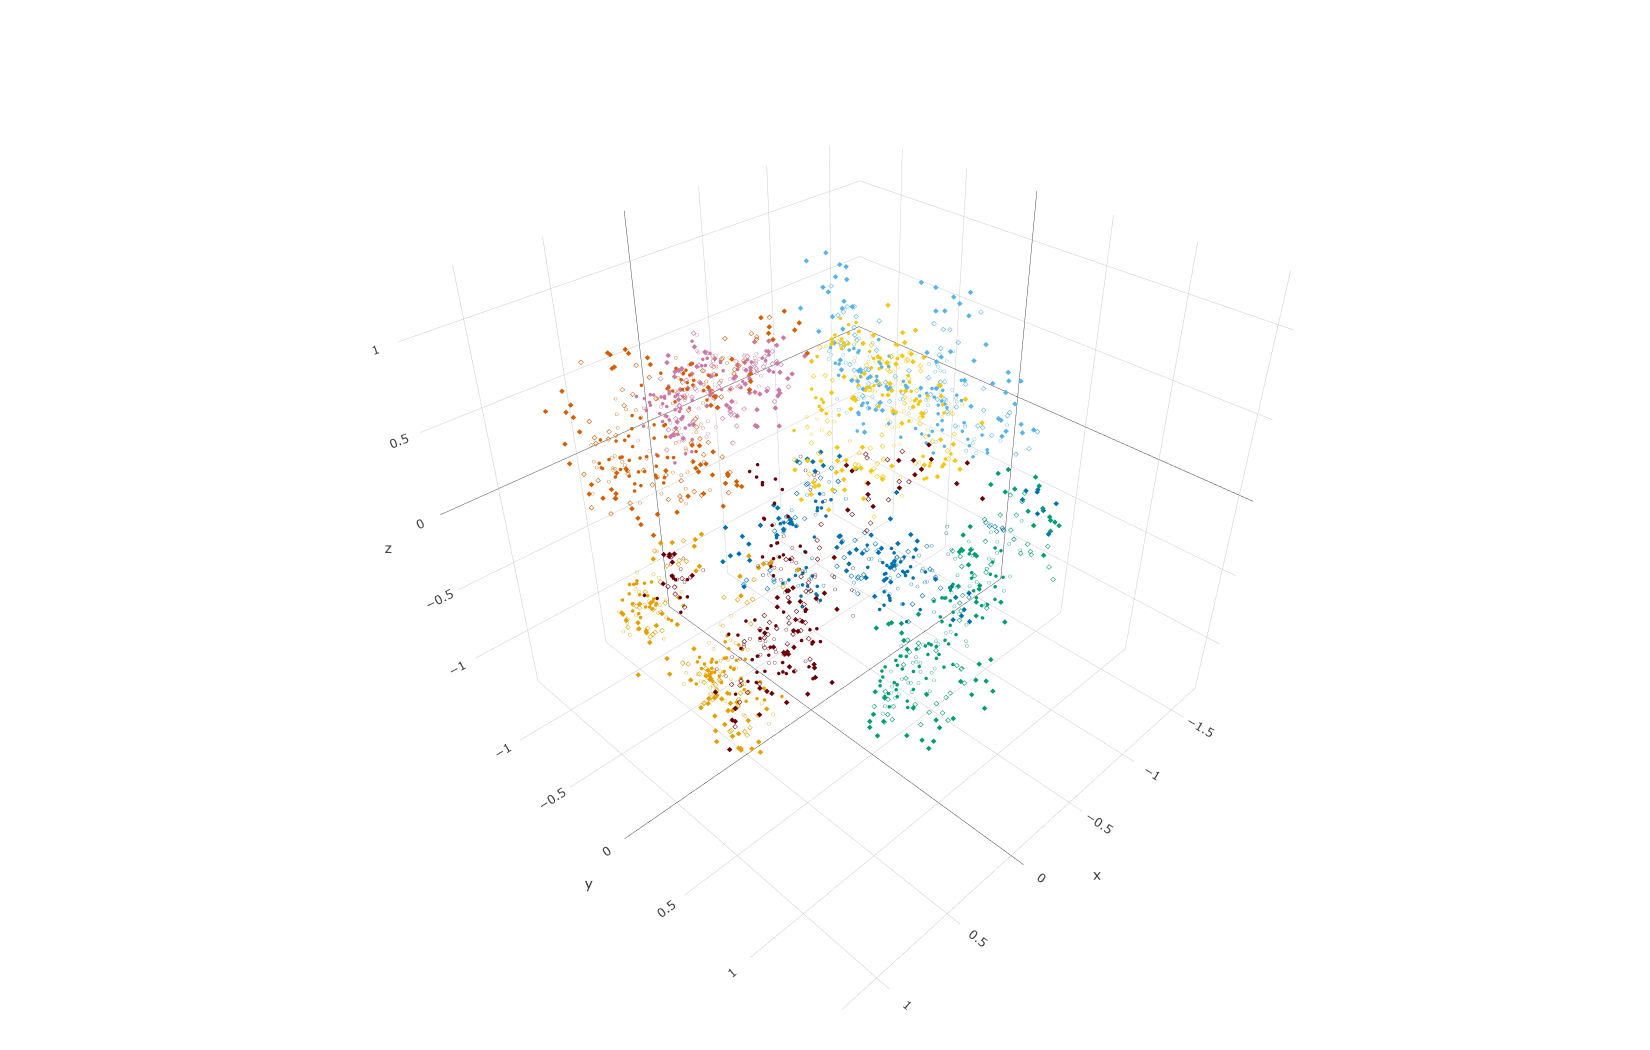
\includegraphics{index_files/figure-pdf/fig-subject-embeddings-a-1.png}

}

\caption{\label{fig-subject-embeddings-a}Final distribution of the 64
embeddings of all the 30 subjects, amounting to 1920 points total.
Embeddings are \textbf{\emph{colored by the species groups}} they
represent. The symbols represent the four imagery groups (Aph. verbal,
spatial, etc.). \textbf{\emph{Interact with the figures to see the
details.}}}

\end{figure}%

\textsubscript{Source:
\href{https://m-delem.github.io/2499-similarity-manuscript/index.qmd.html}{Article
Notebook}}

\phantomsection\label{cell-fig-subject-embeddings-b}
\begin{figure}[H]

\centering{

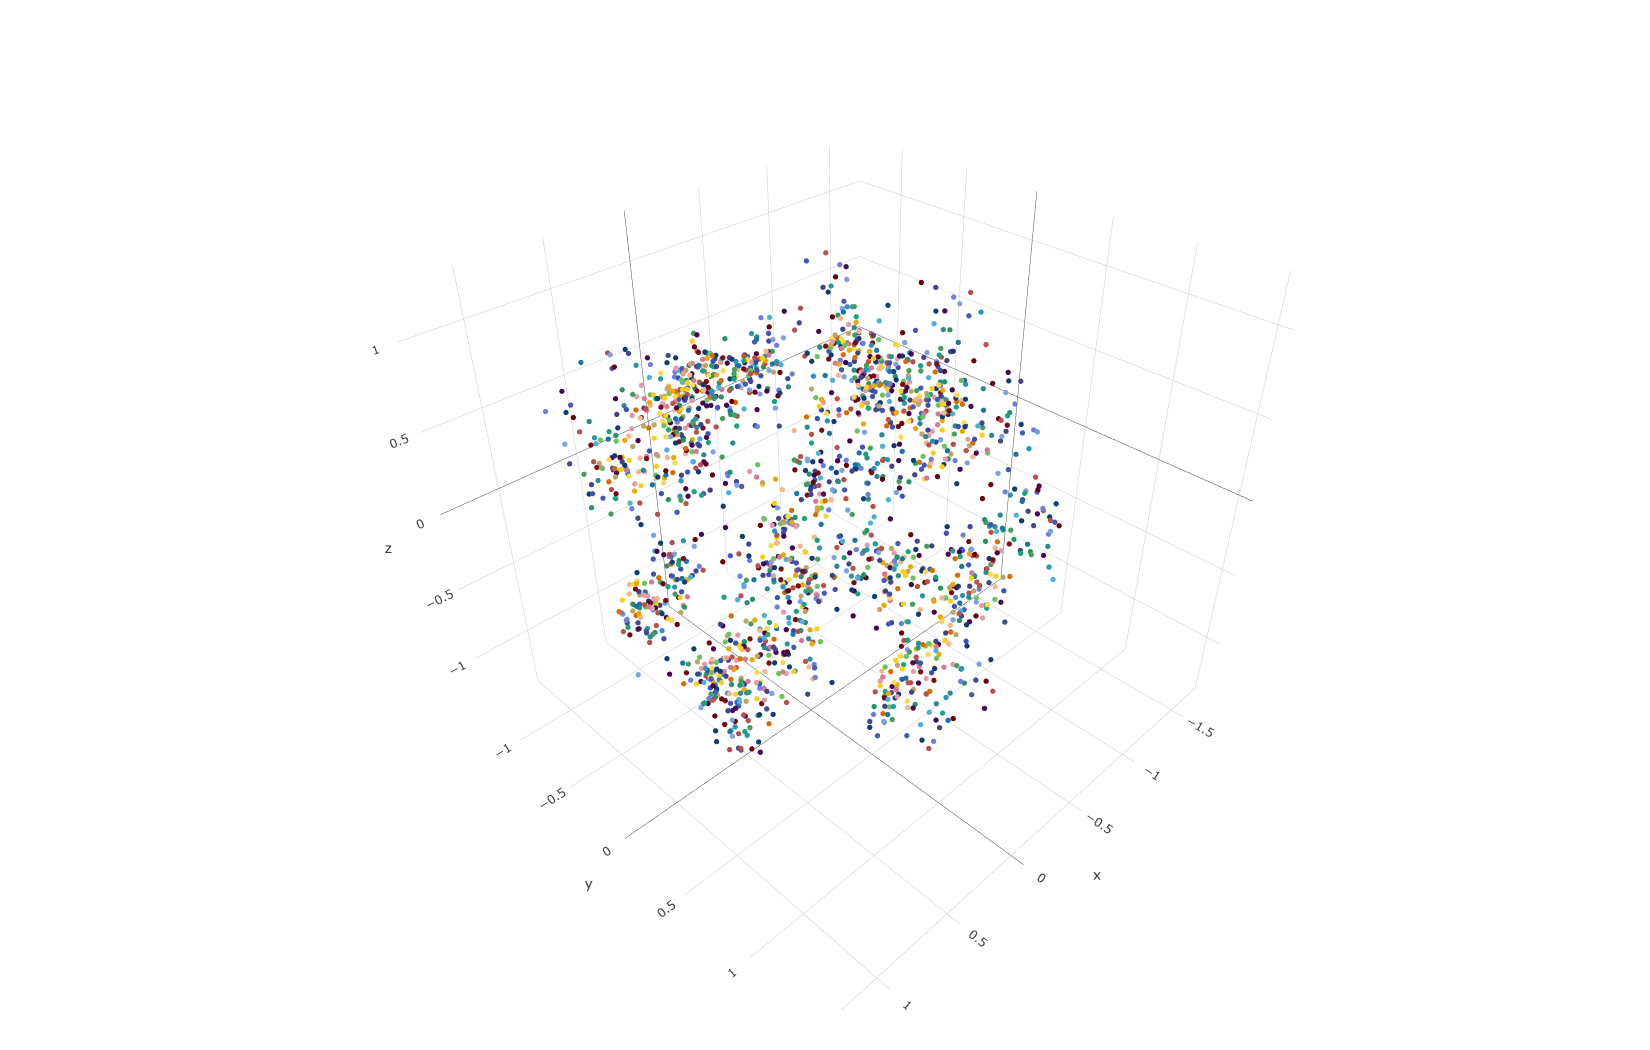
\includegraphics{index_files/figure-pdf/fig-subject-embeddings-b-1.png}

}

\caption{\label{fig-subject-embeddings-b}Final distribution of the 64
embeddings of all the 30 subjects, amounting to 1920 points total.
Embeddings are \textbf{\emph{lored by subject}}. The symbols represent
the four imagery groups (Aph. verbal, spatial, etc.).
\textbf{\emph{Interact with the figures to see the details.}}}

\end{figure}%

\textsubscript{Source:
\href{https://m-delem.github.io/2499-similarity-manuscript/index.qmd.html}{Article
Notebook}}

To feed this data to the algorithm, we'll group the 64 embeddings per
subject in matrices tied to each of them.

\textsubscript{Source:
\href{https://m-delem.github.io/2499-similarity-manuscript/index.qmd.html}{Article
Notebook}}

\subsection{Data analysis: Aligning representational
structures}\label{data-analysis-aligning-representational-structures}

\begin{center}\rule{0.5\linewidth}{0.5pt}\end{center}

\subsection{Simulation summary}\label{simulation-summary}

\citet{kawakita2023}: These results indicate that the difference between
the qualia structures of neuro-typical and atypical participants is
significantly larger than the difference between the qualia structures
of neuro-typical participants.

A notable difference is that greenish colors and reddish colors are
close in the embedding space of color atypical participants while they
are distant in the embedding space of color neurotypical participants.
This structural difference is likely to prevent the unsupervised
alignment between the embeddings of color-neurotypical and atypical
participants even though the correlation coefficient between the
dissimilarity matrices of color neuro-typical and atypical participants
is reasonably high.

For a long time, assessing the similarity of subjective experiences
across participants has been challenging. To address this problem, we
proposed the ``qualia structure'' paradigm, which focuses on
quantitative structural comparisons of subjective experiences. Using an
unsupervised alignment method, we were able to match the qualia
structures of colors and natural objects of different groups of
participants based only on the way the qualia relate to each other,
without using any external labels.

Our results on color qualia structures are consistent with an idea that
the relational properties of color qualia are universally shared by
color-neurotypical individuals. Intriguingly, our results also suggest
that individuals with color-atypical vision may have a different
structure of their color experiences, rather than just failing to
experience a certain subset of colors. Longstanding thought experiments
that challenge the feasibility of inter-subjective color comparisons,
such as individuals with color qualia inversion, should be resolvable
with our relational unsupervised approach. Beyond traditional measures
such as Pearson's correlation coefficient, our method provides a more
fundamental structural characterization of how two structures are
similar or different, which will be crucial for future investigations of
qualia structures across psychological, neuroscientific, and
computational fields.

\section{Feasibility}\label{feasibility}

\section{Conclusion}\label{conclusion}

Modern psychology builds on the relativistic framework of philosophy,
accepting that humans cannot know reality in an absolute sense. Focusing
on relative comparisons, or similarity, is more than a clever
philosophical work-around. similarity is a common currency of perception
and cognition. In addition to operating at all levels of cognition,
similarity---or, more accurately, the second-order isomorphism defined
by a set of similarity relations---has been a powerful tool for
analyzing and comparing psychological spaces.


  \bibliography{references.bib}


\end{document}
